\chapter{Robinson Foulds Metric}
A field, where tree edit distances get applied a lot is the field of computational biology and bioinformatics. Comparing the structure of different RNAs is a classic example of such an application. An even more important one is comparing phylogenetic trees. A phylogenetic tree or evolutionary tree is a rooted branching diagram, that shows the evolutionary connectedness of different species. Multiple species can have recent common ancestor (in the evolutionary sense). This ancestor is represented as a node with an edge to all the descended species. A leaf is called a taxon and is labelled with the species it represents. All in all, one can build one huge phylogenetic tree that represents all life on earth. For the studies of evolutionary biology, scientists often need to compare different evolutionary theories regarding a certain subset of species. Therefore they have to take a look at the structure of the corresponding subtrees and apply some distance measurement on them. \\


\section{Additional Background}
The scientific field of phylogenetics is the field of evolutionary relationships and history among species and groups of organisms. This common ancestry is described as a phylogenetic tree. The taxons, the labels of the leaves of the phylogenetic tree, are hereby the species currently investigated. The interior nodes represent some common ancestor of the investigated species. If we create a rooted phylogenetic tree, then the root would be the common ancestor of all these species. Sometimes the structure can't be fully resolved. This results in so called \textit{multifurcations}, interior nodes of degree higher than three. 
\begin{figure}
	\centering
	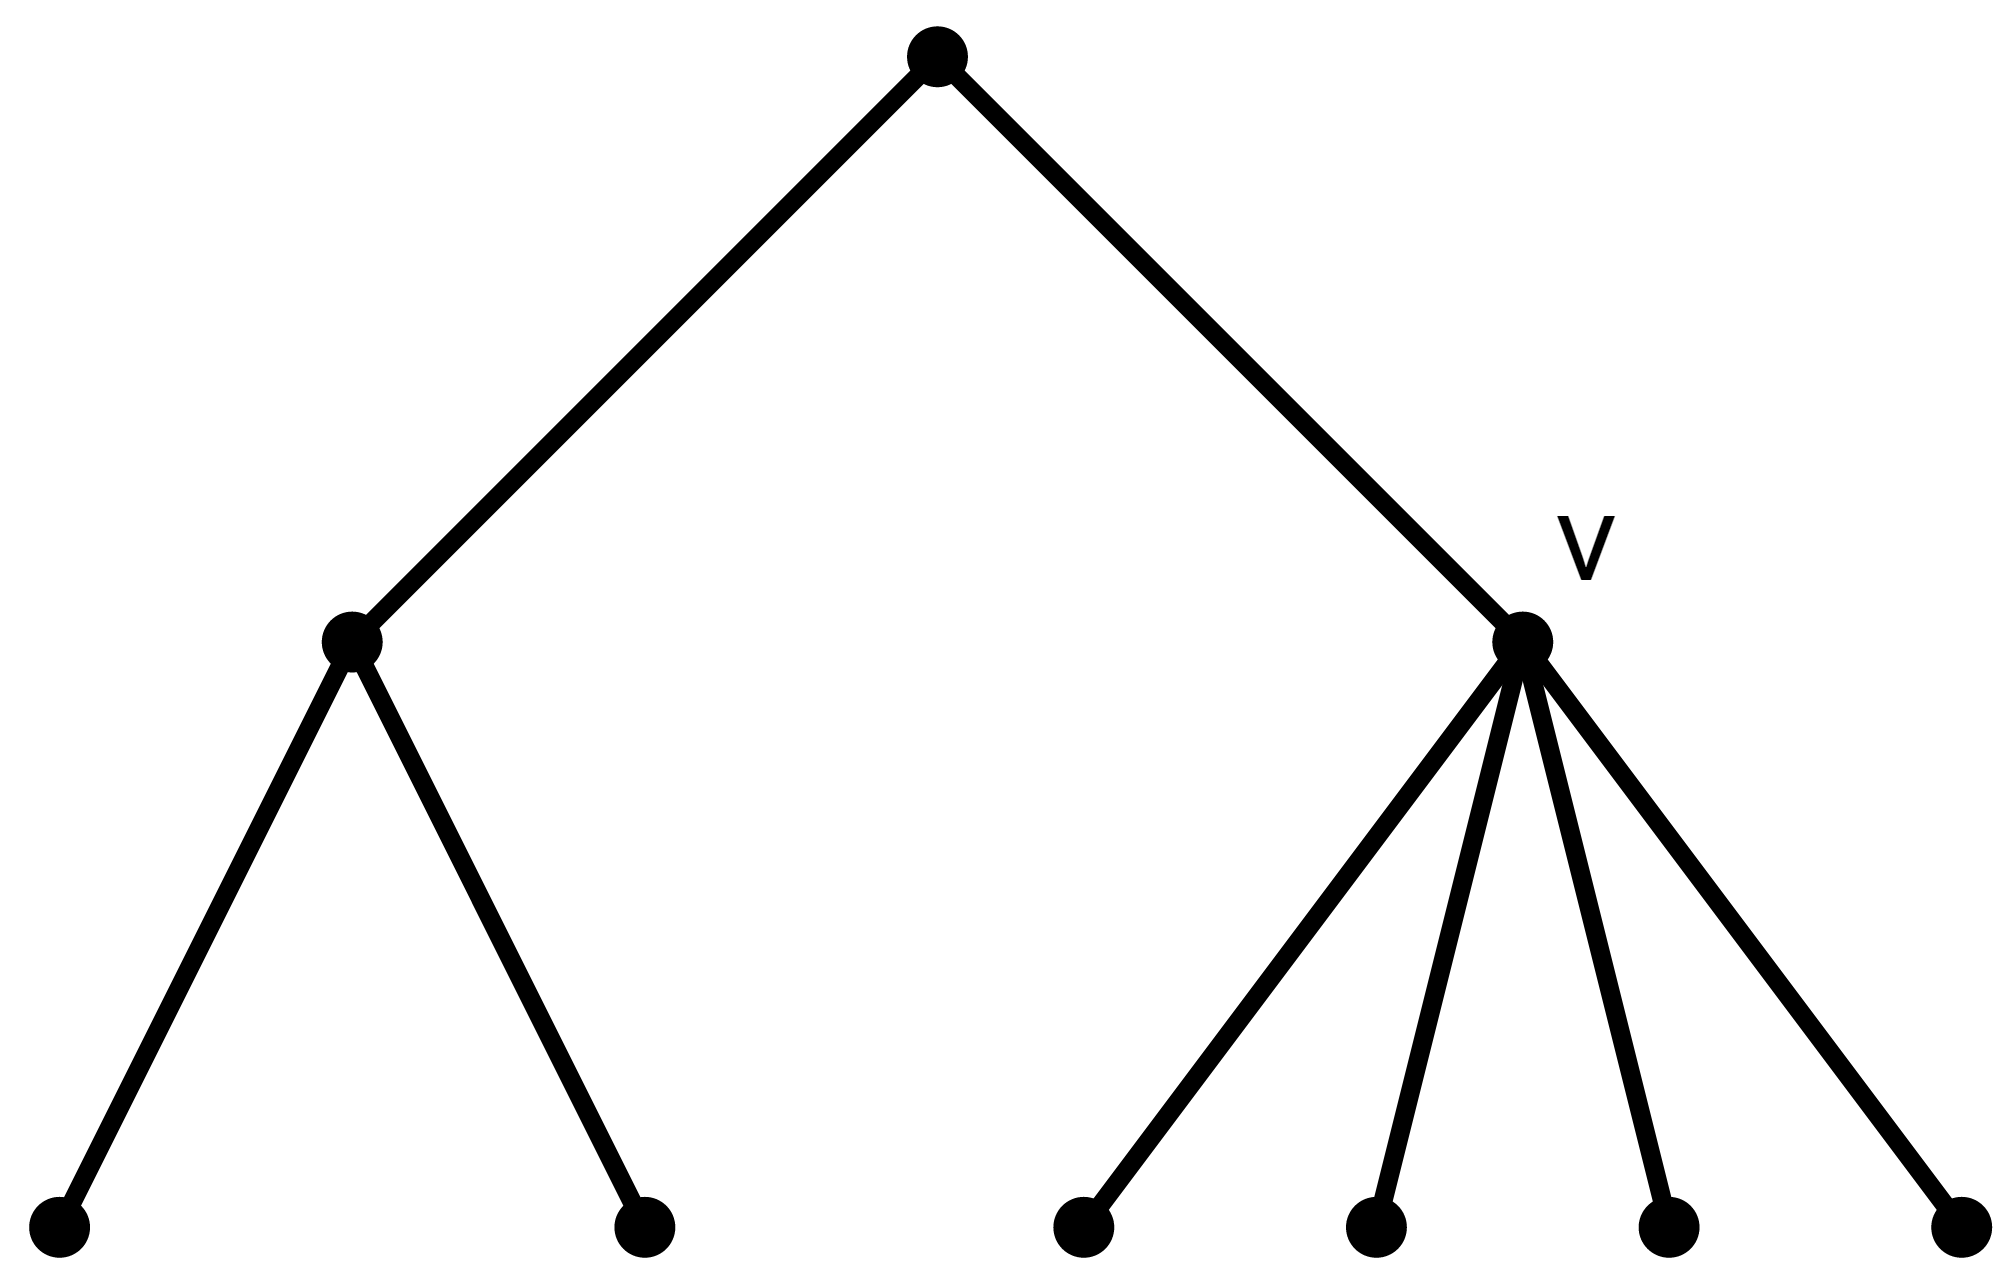
\includegraphics[width=0.4\textwidth]{figures/multifurcation.png}
    \caption{A rooted phylogenetic tree. The node $v$ is a multifurcation since its degree is larger than $3$. The ancestry relations aren't fully resolved for the children of $v$.}
\end{figure}
Multifurcations may occur due to missing data for inferring the phylogeny. Often they appear in consensus trees, when partially contradictory trees were obtained by some methods. A perfectly resolved phylogenetic tree doesn't have any multifurcations implying a binary phylogenetic tree. 

\section{The original metric}
The most commonly used distance measurement was introduced by Robinson and Foulds []. They introduced the term clade, which describes a group of leaves that have a common ancestor which they do not share with any other node.

The Robinson-Foulds metric is quite intuitive and easy to compute. It is the average number of clades that are present in exactly one of the two trees:
\begin{defin}
Let $T_1,T_2$ be two trees with the same set of taxa $X$. Then we define the Robinson-Foulds metric $d_{RF}$ as follows:
\[ d_{RF} := \frac{1}{2}|\mathcal{C}^*(T_1) \bigtriangleup \mathcal{C}^*(T_2)| \]
\end{defin}
\begin{rem}
Assuming that two trees $T_1$,$T_2$ have the same set of taxa $X$ with $n:= |X|$ implies that the number of interior nodes is bounded by $n-1$ for both trees. Furthermore, since we ignore trivial clades, the clade $X$, induced by the tree's root, will be ignored. Thus we end up with a maximum RF-distance of $n-2$ for two trees with the same taxa sets of size $n$.
\end{rem}
Although the Robinson-Foulds metric is commonly used, it has some well known downsides. For example changing the position of a single leaf can yield a new tree having maximal distance from the original one. Let's take a look at Figure~\ref{fig:maxRFdist}. Let $T_1$ be the left tree and $T_2$ be the right one. It is easy to see that the set of clades are the following:
\begin{align*}
\mathcal{C}^*(T_1) &=\{ \{1,...,j\}\;|\;j\in \{2,...,7\}\} \\
\mathcal{C}^*(T_2) &=\{ \{2,...,j\}\;|\;j\in \{3,...,7\}\} \cup \{1,8\}
\end{align*}
Obviously in tree $T_1$ every clade either contains both nodes $1$ and $2$. On the other hand in tree $T_2$ every clade either contains node $1$ or $2$, but never both of them. This implies that 
\begin{align*}
\mathcal{C}^*(T_1) \cap \mathcal{C}^*(T_2) &= \emptyset \\
d_{RF} = \frac{1}{2}|\mathcal{C}^*(T_1) \bigtriangleup \mathcal{C}^*(T_2)| &= \frac{1}{2}(|\mathcal{C}^*(T_1)| + |\mathcal{C}^*(T_2)|) \\
d_{RF} = \frac{1}{2}(6 + 6) = 6
\end{align*}
\begin{figure}[ht!] \label{fig:maxRFdist}
    \begin{subfigure}[b]{0.45\textwidth}
        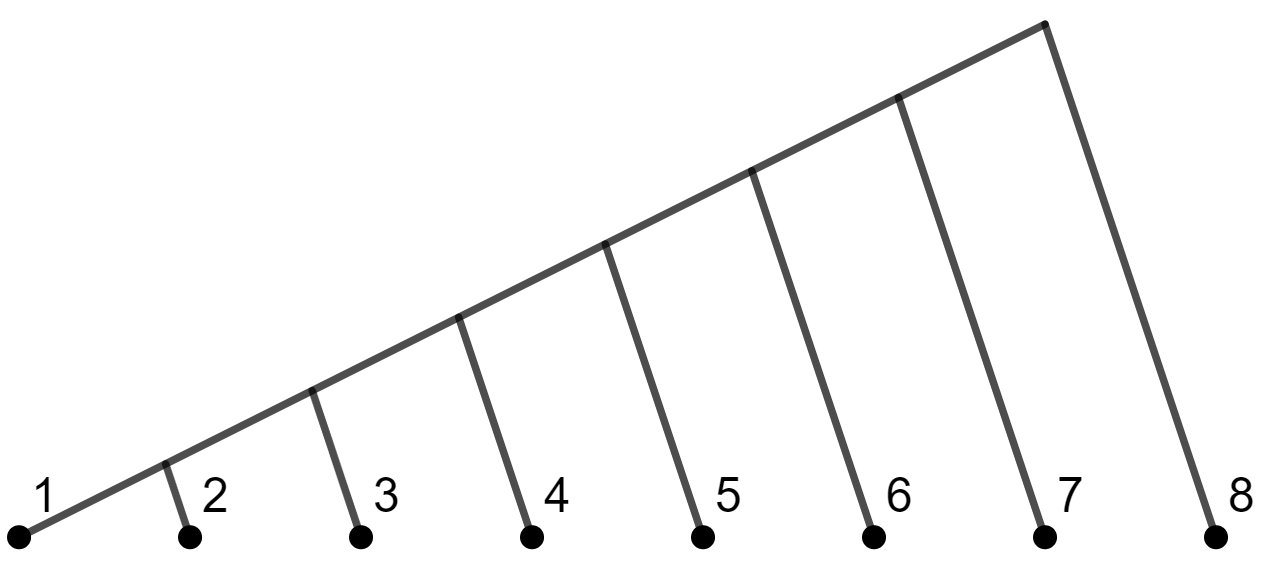
\includegraphics[width=\textwidth]{figures/RF_tree1.jpg}
    \end{subfigure}
    \quad
    \begin{subfigure}[b]{0.45\textwidth}
        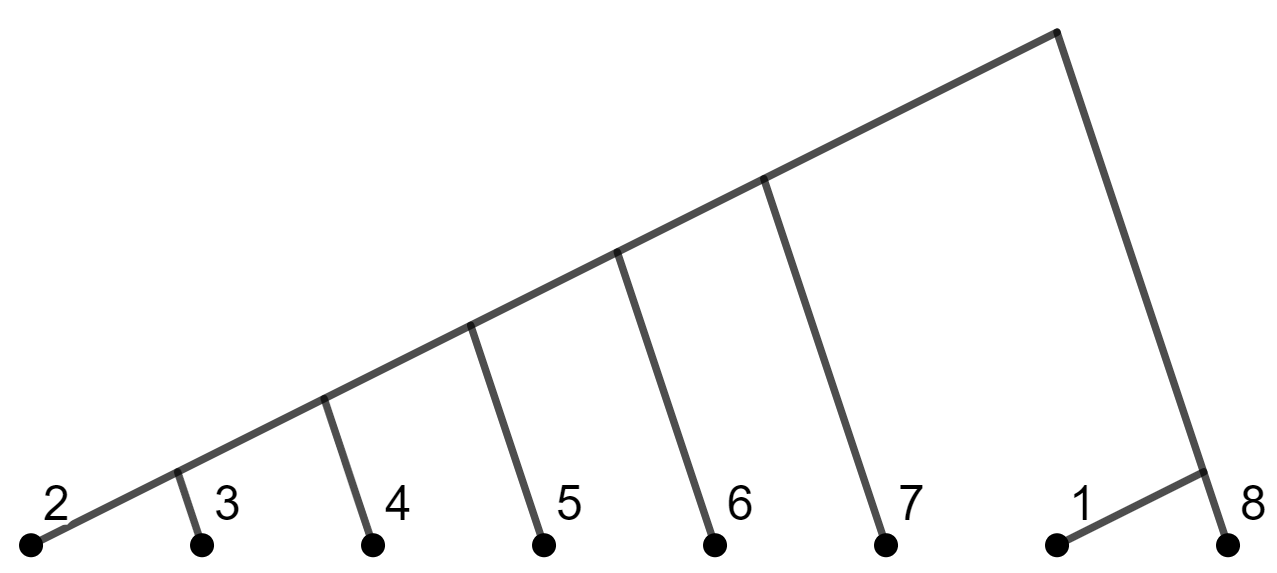
\includegraphics[width=\textwidth]{figures/RF_tree2.jpg}
    \end{subfigure}
    \caption{Two trees having the maximal RF-distance on the set of taxa $\{1,...,8\}$}
\end{figure}
Another big disadvantage is the bad distribution of the distance 
 
\section{The Generalized Robinson Foulds}
To take advantage of structural similarities between $T_1$, $T_2$ Böcker et al.~\cite{Boe} suggested to extend the Robinson Foulds metric. They wanted to relax the condition to just count any clade which appears in the set of clades for one but not both trees. Therefore they matched the clades of the trees and introduced a cost function that measures dissimilarities between two clades. Let $\delta$ be a cost function defined as follows:
$$ \delta: (\mathcal{P}(X) \cup \{\emptyset\}) \times (\mathcal{P}(X) \cup \{\emptyset\}) \mapsto \mathcal{R}_{\geq 0} \cup \{\infty\},$$
where $\mathcal{P}(X)$ denotes the power set of $X$. Now $\delta(C,C')$ measures the dissimilarities between two clades $C$, $C' \subset X$. The value of $delta(C, \emptyset) > 0$ denotes the costs of not matching a clade $C \in \mathcal{C}^*(T_1)$ with a clade in $\mathcal{C}^*(T_2)$. The value $\delta(\emptyset, C')$ is defined analogously.

Let $M \subset \mathcal{C}^*(T_1) \times \mathcal{C}^*(T_2)$ be a matching between the sets of non-trivial clades of $T_1$ and $T_2$. We call a clade $C \in \mathcal{C}^*(T_1)$ unmatched, if $(C, C') \notin M \; \forall C' \in \mathcal{C}^*(T_2)$, analogously for clades of $T_2$. Now we can define the costs $d(M)$ of a matching $M$ as:
$$d(M) := \sum_{(C, C') \in M} \, \delta(C,C') + \sum_{\substack{C \in \mathcal{C}^*(T_1),\\ C\text{ unmatched in }M}} \delta(C, \emptyset) + \sum_{\substack{C' \in \mathcal{C}^*(T_2),\\C'\text{ unmatched in }M}} \delta(\emptyset, C')$$
To see that this is a generalization of the Robinson Foulds, take a look at the following cost function $\delta_{RF}$:
$$\delta_{RF}(C, C') = 
\begin{cases}
	0 & \text{if } C = C' \\
	1 & \text{if } C = \emptyset \text{ or } C' = \emptyset \\
	\infty & \text{if } C \neq C' \text{ and } C \neq \emptyset \neq C'
\end{cases}$$
\begin{lem}\label{lem:costfct}
Let all be given as written above. The task of computing the cheapest matching $M$ can be simplified by the following model: Let $G$ be a complete bipartite graph with node set $V(G) = \mathcal{C}^*(T_1) \dot{\cup} \mathcal{C}^*(T_2)$. For any edge $\{C,C'\} \in E(G)$ let its weight be given by 
\begin{equation} \label{eq:costfct}
\omega(C,C') := \delta(C,\emptyset) + \delta(\emptyset, C') - \delta(C,C').
\end{equation}
Finding a minimal cost matching $M$ of clades is now equivalent to finding a maximal cost matching $M^*$ in $G$. If $\delta$ is a metric, then all weights are positive.
\end{lem}
\begin{proof}
Let $M^*$ be a maximal cost matching in $G$. Then the following implications are trivial:
\begin{gather*}
\sum_{\{C,C'\} \in M^*} \, \omega(C, C') = \max_{M} \, \sum_{\{C,C'\} \in M} \delta(C,\emptyset) + \delta(\emptyset, C') - \delta(C,C') \\
= \max_{M} \, \underbrace{\sum_{C \in \mathcal{C}^*(T_1)} \delta(C,\emptyset)}_{\textit{const. }K_1} - \sum_{\substack{C \in \mathcal{C}^*(T_1),\\ C\text{ unmatched}}} \delta(C,\emptyset) + \underbrace{\sum_{C' \in \mathcal{C}^*(T_2)} \delta(\emptyset, C')}_{\textit{const. }K_2} \\
- \sum_{\substack{C \in \mathcal{C}^*(T_1),\\ C\text{ unmatched}}} \delta(\emptyset, C') - \sum_{\{C,C'\} \in M} \delta(C,C')\\
= K_1 + K_2 + \max_{M} - \bigg( \sum_{\substack{C_1 \in \mathcal{C}^*(T_1),\\ C\text{ unmatched}}} \delta(C, \emptyset) + \sum_{\substack{C \in \mathcal{C}^*(T_1),\\ C\text{ unmatched}}} \delta(\emptyset, C') + \sum_{\{C,C'\} \in M} \delta(C,C') \bigg)\\
= K_1 + K_2 - \min_{M} d(M) = K_1 + K_2 - d(M^*)
\end{gather*}
\end{proof}

Returning to the example above. Assume that the cost function $\delta$ is the symmetric difference between sets:
$$\delta(C_1, C_2) = |C_1 \triangle C_2| = |C_1 \cup C_2| - |C_1 \cap C_2|$$
In this case, the best way to match a clade $\{1,...,j\} \in \mathcal{C}^*(T_1), j \geq 3$ to a clade in $\mathcal{C}^*(T_2)$ is to match it with the clade $\{2,...,j\}$, since its symmetric difference is only $1$. This handles all cases except for the clade $\{1,2\} \in \mathcal{C}^*(T_1)$ and $\{1,8\} \in \mathcal{C}^*(T_2)$. Matching those two clades is better than keeping them unassigned, since:
$$\delta(\{1,2\},\{1,8\}) = 2 < 4 = \delta(\{1,2\},\emptyset) + \delta(\emptyset, \{1,8\})$$
Resulting in a matching of overall costs of $8$.

The minimum matching for the case above show cases a problem with this straight forward approach: The clade $\{1,2\} \in \mathcal{C}^*(T_1) \subset \{1,...,j\} \in \mathcal{C}^*(T_1) \forall j \geq 3$, however this doesn't hold for its matched clade $\{1,8\}$. Therefore we need to concentrate on arboreal matchings:

\begin{defin}\label{def:arboreal}
Let two rooted phylogenetic trees $T_1, T_2$ on the same set of taxa $X$ be given. A matching $M$ on their sets of non-trivial clades is called \textit{arboreal} if for any two edges $\{C_1,C_2\}, \{C_1',C_2'\} \in M$ one of the following cases hold:
\begin{enumerate}
\item $C_1 \subseteq C_1' \wedge C_2 \subseteq C_2'$
\item $C_1' \subseteq C_1 \wedge C_2' \subseteq C_2$
\item $C_1 \cap C_1' = \emptyset \wedge C_2 \cap C_2' = \emptyset$
\end{enumerate}
\end{defin}
\begin{defin}
Let $T_1$ and $T_2$ be two rooted phylogenetic trees on the same set of taxa $X$ and let $\delta$ be a cost function on two subsets of $X$. Furthermore, let $M^*$ to be an arboreal matching between non-trivial clades of $T_1$ and $T_2$ that minimizes the cost function $d(M)$ among all such arboreal matchings $M$. Then we denote the value $d(M^*)$ as the \textit{general Robinson-Foulds distance} between $T_1$ and $T_2$ with respect to $\delta$.
\end{defin} 
\begin{lem}
Let $\delta$ be a cost function as defined above and assume it to be a metric. Then the induced generalized Robinson Foulds distance is a metric on the set of rooted phylogenetic trees on $X$.
\end{lem}
The proof is provided in the full version of the Böcker et al.'s paper~\cite{Boe}.

\subsection{Jaccard-Robinson-Foulds metric}
One specific metric used as a cost function is motivated by the Jaccard index of two sets: 
$$J(A,B) = \frac{|A \cap B|}{|A \cup B|}$$
Generalizing this idea leads to the Jaccard weights of order $k$:
$$\delta_k(C_1,C_2) = 1 - (\frac{|C_1 \cap C_2|}{|C_1 \cup C_2|}^k$$
For completeness $\delta_k(\emptyset, \emptyset)=0 \, \forall k$. The induced generalized Robinson Foulds metric is called Jaccard-Robinson-Foulds metric of order $k$ and is denoted by $d_{JRF}^{(k)}(T_1,T_2)$.\\
For $k \to \infty$ the $d_{JRF}^{(k)}$ converges to the inverse Kronecker delta:
$$\delta_k(C_1,C_2) =
\begin{cases}
0 & \text{if } C_1 = C_2 \\
1 & \text{if } C_1 \neq C_2
\end{cases}$$
This suggests that Jaccard-Robinson-Foulds metric converges to the Robinson Foulds metric.

\subsection{Computational Complexity}
In their paper Böcker et al. demonstrate a polynomial reduction from the $(3,4)$-SAT problem to the problem of finding a minimal cost arboreal matching, even if the cost function $\delta$ is a metric. The $(3,4)$-SAT is the problem of finding a satisfying assignment for a Boolean formula in which every clause consists of exactly $3$ literals and any variable occurs $4$ times.\\
The authors of the above mentioned paper were able to construct a minimum arboreal matching instance $I$ for any Boolean formula $\phi \in (3,4)$-SAT. If the problem $I$, using the symmetric difference as cost function, admits a solution with a value smaller than a certain value, the original problem of finding a correct assignment for $\phi$ has a solution. For more details we suggest to read the original paper~\cite{Boe}. 
\begin{thm}
For an instance of the arboreal matching using the symmetric difference as cost function $\delta$ and an integer $k$, it is $NP$-complete whether there exists an arboreal matching of cost at most $k$.
\end{thm}

\subsection{An Integer Linear Program}
One way to approach an $\mathcal{NP}$-complete problem is to introduce an integer linear program and try to find an assignment that minimizes the overall cost as much as possible. Therefore Böcker et al. set up an integer linear programming formulation to find a minimum cost arboreal matching.\\
Let two rooted phylogenetic trees $T_1 = (V_1,E_1)$ and $T_2 = (V_2,E_2)$ and a cost function $\delta: \mathcal{C}(T_1 \times \mathcal{C}(T_2) \mapsto \mathbb{R}_{\geq 0}$ be given. We number the clades in $\mathcal{C}(T_i)$ from 1 to $|V_i|$ for $i \in \{1,2\}$. Then the indicator variable $x_i,j$ represents whether the $i$-th clade $C_i$ in $\mathcal{C}(T_1)$ is matched with the $j$-th clade $C'_j$ in $\mathcal{C}(T_2)$. We use the cost function introduced in equation~(\ref{eq:costfct}) to find a minimum cost matching while maximizing the sum of the cost function. To recapitulate, the value for $\omega(C_i,C'_j)$ is:
$$\omega(C_i,C'_j) = \delta(C_i,\emptyset) + \delta(\emptyset, C'_j) - \delta(C_i,C'_j)$$
We also have to make sure that the assignment we receive satisfies the conditions for an arboreal matching. Therefore we introduce the set $\mathcal{I}$ with the following properties:
\begin{equation*}
\mathcal{I} := \bigg\{ \{(i,j), (k,l)\} \, \Big| \, \parbox{9.8cm}{The edges $(C_i, C'_j)$ and $(C_k, C'_l)$ violate the conditions
\\for arboreal matchings defined in Definition~\ref{def:arboreal}} \bigg\}
\end{equation*}
Now we can formulate the linear program:
\begin{align}
\max &\sum_{i=1}^{|V_1|} \sum_{j=1}^{|V_2|} \; \omega(C_i, C'_j) x_{i,j} \label{eq:max} \\
\text{s.t.} &\sum_{j=1}^{|V_2|} \; x_{i,j} \leq 1 & \forall i \in \{1,...,|V_1|\} \label{eq:V_1} \\
&\sum_{i=1}^{|V_1|} \; x_{i,j} \leq 1 & \forall j \in \{1,...,|V_2|\} \label{eq:V_2} \\
&x_{i,j} + x_{k,l} \leq 1 & \forall \{(i,j), (k,l)\} \in \mathcal{I} \label{eq:arb} \\
&x_{i,j} \in \{0,1\} & \forall i \in \{1,...,|V_1|\}, \forall j \in \{1,...,|V_2|\} \label{eq:int}
\end{align}
\begin{rem} Here we will give a short summary why this linear program describes the optimal solution for the task of finding a minimum cost arboreal matching. Most of the work has already been done in this chapter.\\
First and foremost, the restriction to integer decision variables in Equation~(\ref{eq:int}) ensures, that we either choose an edge to be in the matching or not. Thus we indeed get a set of edges. Furthermore Equations~(\ref{eq:V_1}) and~(\ref{eq:V_2}) restricts the chosen set of edges to be a (not necessarily complete) matching. Last but not least, because of Equation~(\ref{eq:arb}) we can be certain that the matching we end up with is a an arboreal matching, since we constructed the set $\mathcal{I}$ exactly this way. As proven in Lemma~\ref{lem:costfct}, the arboreal matching of maximum cost with respect to the cost function~(\ref{eq:max}) is an arboreal matching that minimizes the generalized Robinson-Foulds distance $d(M)$.
\end{rem}